%%%%%%%%%%%%%%%%%%%%%%%%%%%%%%%%%%%%%%%%%
% Beamer Presentation
% LaTeX Template
% Version 1.0 (10/11/12)
%
% This template has been downloaded from:
% http://www.LaTeXTemplates.com
%
% License:
% CC BY-NC-SA 3.0 (http://creativecommons.org/licenses/by-nc-sa/3.0/)
%
%%%%%%%%%%%%%%%%%%%%%%%%%%%%%%%%%%%%%%%%%

%----------------------------------------------------------------------------------------
%	PACKAGES AND THEMES
%----------------------------------------------------------------------------------------

\documentclass{beamer}

\mode<presentation> {

% The Beamer class comes with a number of default slide themes
% which change the colors and layouts of slides. Below this is a list
% of all the themes, uncomment each in turn to see what they look like.

%\usetheme{default}
%\usetheme{AnnArbor}
%\usetheme{Antibes}
%\usetheme{Bergen}
%\usetheme{Berkeley}
%\usetheme{Berlin}
%\usetheme{Boadilla}
%\usetheme{CambridgeUS}
%\usetheme{Copenhagen}
\usetheme{Darmstadt}
%\usetheme{Dresden} %used at CoE Frontier
%\usetheme{Frankfurt}
%\usetheme{Goettingen}
%\usetheme{Hannover}
%\usetheme{Ilmenau}
%\usetheme{JuanLesPins}
%\usetheme{Luebeck}
%\usetheme{Madrid}
%\usetheme{Malmoe}
%\usetheme{Marburg}
%\usetheme{Montpellier}
%\usetheme{PaloAlto}
%\usetheme{Pittsburgh}
%\usetheme{Rochester}
%\usetheme{Singapore}
%\usetheme{Szeged}
%\usetheme{Warsaw}

% As well as themes, the Beamer class has a number of color themes
% for any slide theme. Uncomment each of these in turn to see how it
% changes the colors of your current slide theme.

%\usecolortheme{albatross}
%\usecolortheme{beaver}
%\usecolortheme{beetle}
%\usecolortheme{crane}
%\usecolortheme{dolphin}
%\usecolortheme{dove}
%\usecolortheme{fly}
%\usecolortheme{lily}
%\usecolortheme{orchid}
%\usecolortheme{rose}
%\usecolortheme{seagull}
%\usecolortheme{seahorse}
%\usecolortheme{whale}
%\usecolortheme{wolverine}

%\setbeamertemplate{footline} % To remove the footer line in all slides uncomment this line
%\setbeamertemplate{footline}[page number] % To replace the footer line in all slides with a simple slide count uncomment this line

%\setbeamertemplate{navigation symbols}{} % To remove the navigation symbols from the bottom of all slides uncomment this line

%to set number for figure
\setbeamertemplate{caption}[numbered]

}

\usepackage{listings}
\usepackage{color}
 
\definecolor{codegreen}{rgb}{0,0.6,0}
\definecolor{codegray}{rgb}{0.5,0.5,0.5}
\definecolor{codepurple}{rgb}{0.58,0,0.82}
\definecolor{backcolour}{rgb}{0.95,0.95,0.92}
 
\lstdefinestyle{mystyle}{
    backgroundcolor=\color{backcolour},   
    commentstyle=\color{codegreen},
    keywordstyle=\color{magenta},
    numberstyle=\tiny\color{codegray},
    stringstyle=\color{codepurple},
    basicstyle=\footnotesize, %\tiny, \small, \footnotesize
    breakatwhitespace=false,         
    breaklines=true,                 
    captionpos=b,                    
    keepspaces=true,                 
    numbers=left,                    
    numbersep=5pt,                  
    showspaces=false,                
    showstringspaces=false,
    showtabs=false,                  
    tabsize=2
}
 
\lstset{style=mystyle}

\usepackage{hyperref}
\usepackage{lipsum}
\usepackage{graphicx} % Allows including images
\usepackage{booktabs} % Allows the use of \toprule, \midrule and \bottomrule in tables

%My personal package
%\usepackage{tikz}

%% Knuths smile box from 
%\centerline{\bf Stable Husbands}
%\bigskip
%\centerline{\sl Donald E. Knuth, Rajeev Motwani, and Boris Pittel}
%\centerline{\sl  Computer Science Department, Stanford University}
\def\pfbox % new experimental version (DEK, November 88)
{{\ooalign{\hfil\lower.06ex % a smiley face
 \hbox{$\scriptscriptstyle -$}\hfil\crcr
 \hfil\lower.7ex\hbox{\"{}}\hfil\crcr
 \mathhexbox20D}}}

%----------------------------------------------------------------------------------------
%	TITLE PAGE
%----------------------------------------------------------------------------------------

\title[IPP]{Installation to Python 3 Programming: Installation and Basic Coding} % The short title appears at the bottom of every slide, the full title is only on the title page

\author{Muhammad Izham} % Your name
\institute[Universiti Malaysia Perlis] % Your institution as it will appear on the bottom of every slide, may be shorthand to save space
{
Universiti Malaysia Perlis \\ % Your institution for the title page
\medskip
\textit{izham@unimap.edu.my} \\
\textit{sugita5019@gmail.com} \\ %email

%Check out my templates for simple stuffs

\textit{https://github.com/izham-sugita}
}
\date{} % Date, can be changed to a custom date

\begin{document}

\begin{frame}
\titlepage % Print the title page as the first slide
\end{frame}

\begin{frame}
\begin{center}
\begin{figure}

\includegraphics[scale=0.25]{python-logo.png}
\caption{Python's logo.}
\end{figure}
\end{center}
\end{frame}


%----------------------------------------------------------------------------------------
%	PRESENTATION SLIDES
%----------------------------------------------------------------------------------------

%------------------------------------------------
\section{Warming up} 

\begin{frame}
\frametitle{Before we get started...}
\begin{center}
\begin{figure}
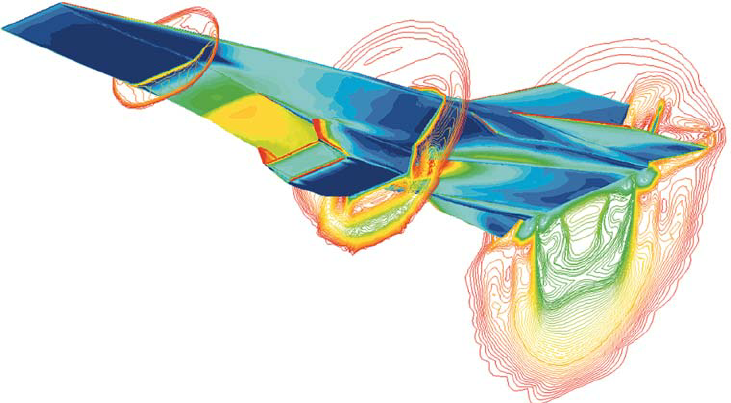
\includegraphics[width=0.3\textwidth]{CFD-NASA-HyperX.png}
\caption{CFD result of HyperX at Mach 7 from NASA}
\end{figure}
\end{center}

\begin{itemize}
\item Basic tool for programming $\longrightarrow$ A good editor.
\item For Windows $\longrightarrow$ geany, notepad++
\item For Linux $\longrightarrow$ emacs, vi 
\end{itemize}

\end{frame}


\begin{frame}
\frametitle{A Little Background}
%\lipsum[1]

\begin{itemize}
\item Created by: Guido van Rossum, 1989-1991
\item Why: The creator wanted something easy to use.
\item Is it really that easy? Yes (and no)
\item Very readable with little memory management.
\item \url{https://people.sc.fsu.edu/~jburkardt/}
\item \url{https://docs.python.org/3/tutorial/index.html}
\item \url{https://www.tutorialsteacher.com/python}
\item \url{https://www.w3schools.com/python/default.asp}
\item \url{https://www.tutorialspoint.com/python/} $\longleftarrow$ great place to start.
\end{itemize}

\end{frame}

\begin{frame}
\frametitle{A Little More About Python}

\begin{itemize}
\item Python2 $\longrightarrow$ Python3; support for Python2 will end 2020.
\item This workshop is exclusively on Python3 $\longrightarrow$ refer to just Python
\item Python is fully object oriented. Everything is considered object.
\item Famous for AI and machine learning $\longrightarrow$ Pytorch, Keras, TensorFlow
\item Interpreter language but can be compiled $\longrightarrow$ Cython, Numba
\item Very well documented. Every module/libraries are documented online.
\item Package management by package installer $\longrightarrow$ pip, pip3
\item pip $\longrightarrow$ \url{https://pypi.org/project/pip/}
\item \textbf{Py}thon \textbf{P}ackage \textbf{I}ndex $\longrightarrow$ pypi, \url{https://pypi.org/}
\item \url{https://github.com/} $\longleftarrow$ another place to look.
\end{itemize}

\end{frame}

\begin{frame}
\frametitle{About Anaconda}
\begin{itemize}
\item No, its not a different programming language.
\item Anaconda is a \emph{complete environment} for Python programming.
\item Most major scientific package (NumPy, SciPy etc) are included.
\item Package installer \emph{conda}
\lstinputlisting[language=bash, firstline=5, lastline=5, numbers=none]{./install-commands.txt}
\item \url{https://www.anaconda.com/}
\end{itemize}

\end{frame}
\begin{frame}[fragile]
\frametitle{About programming}
\begin{figure}
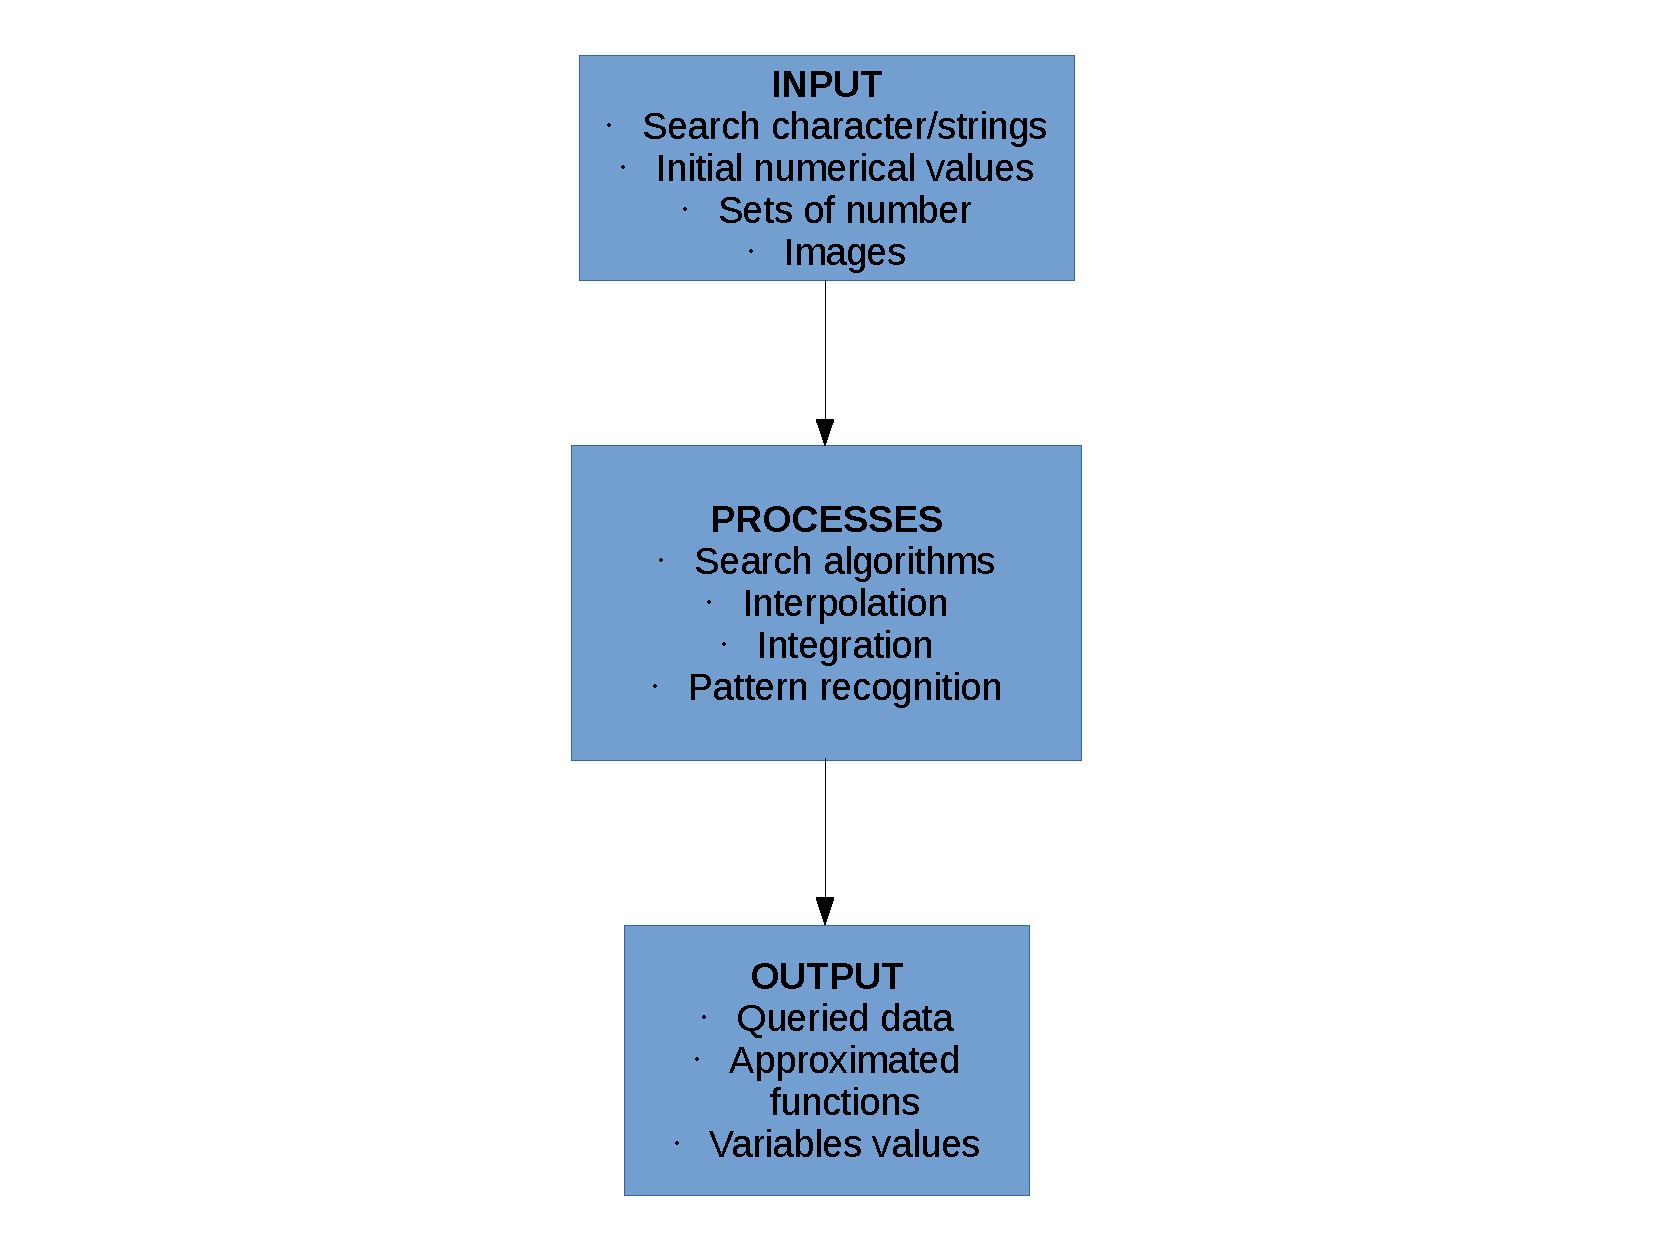
\includegraphics[width=0.8\linewidth]{ProgrammingFlow.pdf}
\end{figure}
\end{frame}

\begin{frame}[fragile]
\frametitle{About programming}
\begin{itemize}
\item Coding paradigm
	\begin{itemize}
	\item programming language == English (sorry, Mandarin not required)
	\item syntax is based on English
	\item coding is a reduction of English instructions
	\end{itemize}

\item Syntax must be remembered
	\begin{itemize}
	\item read the manual $\longrightarrow$ documentations are vital
	\item memorize THE MOST COMMONLY USED syntax only
	\item good algorithm will always beats bad algorithm
	\end{itemize}		

\item I don't remember every syntax so you have to bare with me $\LARGE \pfbox$

\end{itemize}

\end{frame}

\begin{frame}
\frametitle{Installation}

\begin{itemize}
\item Download from \url{https://www.python.org/}
\item For Ubuntu download from repository:\lstinputlisting[language=bash, firstline=1, lastline=1, numbers=none]{./install-commands.txt}

\item For Windows, download from \url{https://www.python.org/downloads/windows/}

\item For Ubuntu installing packages:\lstinputlisting[language=bash, firstline=2, lastline=2, numbers=none]{./install-commands.txt}

\item For Windows installing packages if $C:\backslash Python\backslash Scripts \backslash$ is in the path:\lstinputlisting[language=bash, firstline=3, lastline=3, numbers=none]{./install-commands.txt}

\item For Windows installing packages:\lstinputlisting[language=bash, firstline=4, lastline=4, numbers=none]{./install-commands.txt}

%C:\Python\Scripts

\end{itemize}

\end{frame}


%------------------------------------------------
\section{Code snippets}
%------------------------------------------------
\begin{frame}
\Huge{\centerline{Simple Snippets}}
\end{frame}

\begin{frame}[fragile]
\frametitle{Hello, Python!}
\newcommand{\newfilename}{py-hello.py}
\begin{itemize}
\item Symbols to remember.
\lstinputlisting[language=Python, firstline=1, lastline=15]{../py-hello.py}
\end{itemize}
file: \newfilename
\end{frame}

\begin{frame}[fragile]
\frametitle{Hello, Python!}
\newcommand{\newfilename}{py-hello.py}
\begin{itemize}
\item The print() function.
\lstinputlisting[language=Python, firstline=17, lastline=27]{../py-hello.py}
\end{itemize}
file: \newfilename
\end{frame}

\begin{frame}[fragile]
\frametitle{Basic I/O including files.}
\newcommand{\newfilename}{py-basic-io.py}
\begin{itemize}
\item Basic I/O from terminal.
\lstinputlisting[language=Python, firstline=1, lastline=11]{../py-basic-io.py}
\end{itemize}
file: \newfilename
\end{frame}

\begin{frame}[fragile]
\frametitle{Basic I/O including files.}
\newcommand{\newfilename}{py-file-io.py}
\begin{itemize}
\item Write to file and close.
\lstinputlisting[language=Python, firstline=1, lastline=3]{../py-file-io.py}

\item Write to file with different access mode.
\lstinputlisting[language=Python, firstline=5, lastline=12]{../py-file-io.py}
\end{itemize}
file: \newfilename
\end{frame}

\begin{frame}[fragile]
\frametitle{Loop in Python}
\begin{itemize}
\item for-loop 
\lstinputlisting[language=Python, firstline=11, lastline=16]{../py-loop.py}
\end{itemize}
\end{frame}

\begin{frame}[fragile]
\frametitle{Loop in Python}
\begin{itemize}
\item Loop with string data.
\lstinputlisting[language=Python, firstline=24, lastline=26]{../py-loop.py}
\end{itemize}
\end{frame}

\begin{frame}[fragile]
\frametitle{Loop in Python}
\newcommand{\newfilename}{py-while.py}

\begin{itemize}
\item while-loop.
\lstinputlisting[language=Python, firstline=1, lastline=11]{../py-while.py}
\end{itemize}
file: \newfilename
\end{frame}

\section{Application examples}
\begin{frame}
\Huge{\centerline{Applications: Important Tools}}
\Huge{\centerline{and Sample Codes}}
\end{frame}

\subsection{The Most Common Modules}

\begin{frame}[fragile]
\frametitle{NumPy module}

\begin{itemize}
\item Specific module for numerical simulations.
\item Very excellent for array manipulation.
\item Documentation from \url{https://www.numpy.org/}
\end{itemize}

%\newcommand{\newfilename}{py-matplotlib.py}
%\lstinputlisting[language=Python, firstline=1, lastline=7]{../py-matplotlib.py}
%file: \newfilename

\end{frame}

%-------------------------------------------------------------------------------

\begin{frame}[fragile]
\frametitle{SciPy module}

\begin{itemize}
\item Scientific calculations module.
\item Lots of functions for scientific computation.
\item Documentation from \url{https://www.scipy.org/}
\item Specific manuals \url{https://docs.scipy.org/doc/scipy-1.3.0/reference/}
\end{itemize}

%\newcommand{\newfilename}{py-matplotlib.py}
%\lstinputlisting[language=Python, firstline=1, lastline=7]{../py-matplotlib.py}
%file: \newfilename

\end{frame}

%--------------------------------------------------------------------------------

\begin{frame}[fragile]
\frametitle{Matplotlib module}

\begin{itemize}
\item Very efficient module for plotting almost everything.
\item Capable for plotting graphs and images.
\item Documentation from \url{https://matplotlib.org/3.1.0/index.html}
\end{itemize}

\newcommand{\newfilename}{py-matplotlib.py}
\lstinputlisting[language=Python, firstline=1, lastline=7]{../py-matplotlib.py}
file: \newfilename

\end{frame}

%-------------------------------------------------------------------------------

\begin{frame}[fragile]
\frametitle{pandas module}

\begin{itemize}
\item Python data analysis module.
\item The go-to module for data analysis.
\item Documentation from \url{https://pandas.pydata.org/}
\end{itemize}

\end{frame}

%-------------------------------------------------------------------------------

\begin{frame}[fragile]
\frametitle{Numba module}

\begin{itemize}
\item Python module for high performance computing.
\item Just-In-Time (JIT) compiler for faster computation.
\item Documentation from \url{https://numba.pydata.org/}
\end{itemize}

%\newcommand{\newfilename}{py-matplotlib.py}
%\lstinputlisting[language=Python, firstline=1, lastline=7]{../py-matplotlib.py}
%file: \newfilename

\end{frame}

%-------------------------------------------------------------------------------

\begin{frame}[fragile]
\frametitle{*Numba with CUDA}

\begin{itemize}
\item GPU computing implementation using Numba-CUDA.
\item Very common in AI and DeepLearning implementation.
\item Example code:
\end{itemize}

\newcommand{\newfilename}{py-numba-cuda.py}
\lstinputlisting[language=Python, firstline=1, lastline=4]{../py-numba-cuda.py}
file: \newfilename

*Special settings are required.
\end{frame}
%---------------------------------------------------------------------------------

\begin{frame}[fragile]
\frametitle{Numba with CUDA}
\newcommand{\newfilename}{py-numba-cuda.py}

\begin{itemize}
\item Example output for device detection.
\end{itemize}
\begin{figure}
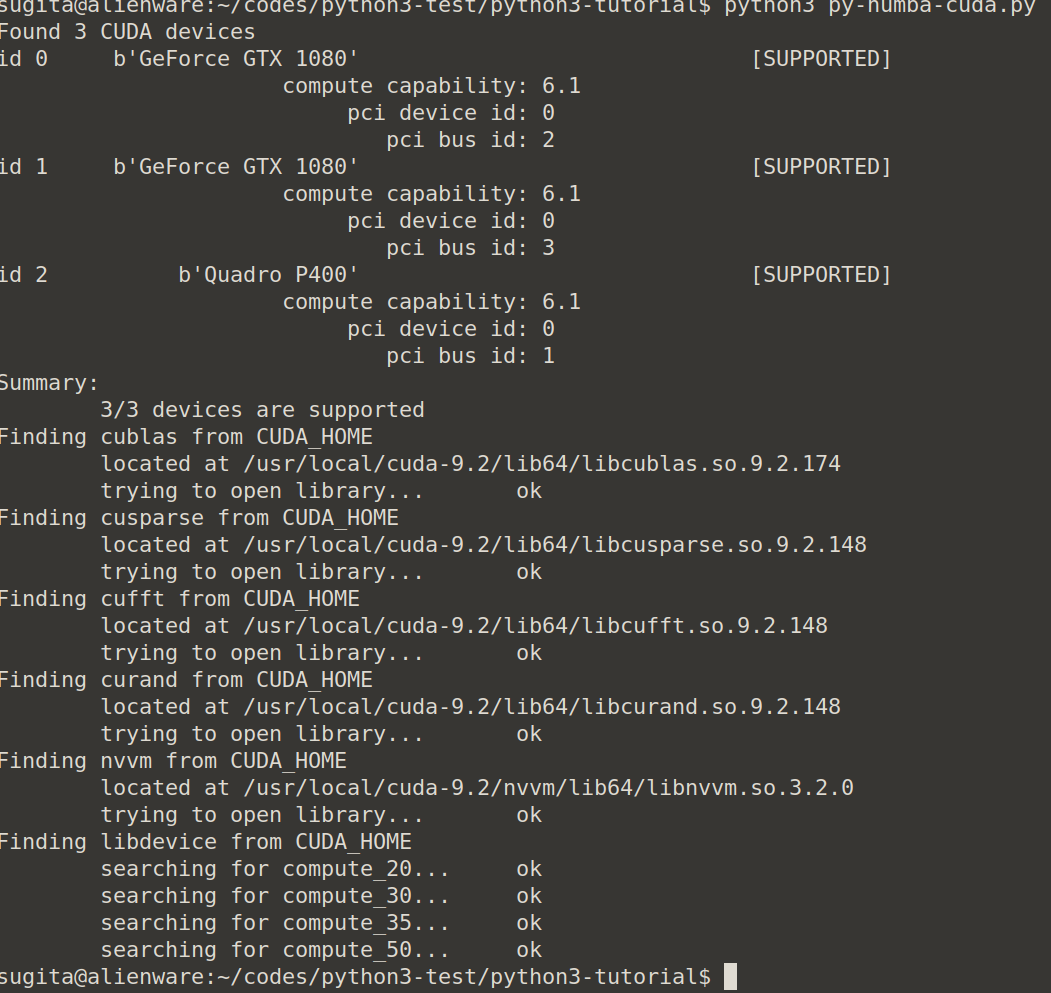
\includegraphics[width=0.5\textwidth]{dev-numba.png}
\caption{Numba's device detection.}
\end{figure}
file: \newfilename
\end{frame}

%-------------------------------------------------------------------------------

\begin{frame}[fragile]
\frametitle{Numba with CUDA}
\begin{itemize}
\item Example for CUDA kernel using numba
\end{itemize}
\newcommand{\newfilename}{py-numba-cuda-mxm.py}
\lstinputlisting[language=Python, firstline=6, lastline=16]{../py-numba-cuda-mxm.py}
file: \newfilename
\end{frame}

%-------------------------------------------------------------------------------

\subsection{Finite Difference Method}
\begin{frame}[fragile]
\frametitle{Finite difference method for heat equation}
\newcommand{\newfilename}{py-precise-loop.py}
\begin{itemize}
\item The 1D equation : $\frac{\partial T}{\partial t} = \kappa \frac{\partial^2 T}{\partial x^2}$
\lstinputlisting[language=Python, firstline=1, lastline=16]{../fdm-py/1D-heat-numba.py}
\end{itemize}
\end{frame}


\subsection{Monte-Carlo Simulation}
\begin{frame}[fragile]
\frametitle{Monte-Carlo Simulation}
\newcommand{\newfilename}{py-MonteCarlo.py}
\begin{itemize}
\item Monte-Carlo simulation to calculate the value of $\pi$
\item The code below shows a straightforward implementation.
\lstinputlisting[language=Python, firstline=20, lastline=30]{../py-MonteCarlo.py}
\end{itemize}
file: \newfilename
\end{frame}

\begin{frame}[fragile]
\frametitle{Monte-Carlo Simulation}
\newcommand{\newfilename}{py-MonteCarlo.py}
\begin{itemize}
\item With Numba jit
\lstinputlisting[language=Python, firstline=3, lastline=14]{../py-MonteCarlo.py}
\end{itemize}
file: \newfilename
\end{frame}

\begin{frame}[fragile]
\frametitle{Monte-Carlo Simulation}
\begin{itemize}
\item Computation time Numba vs Normal script
\begin{figure}
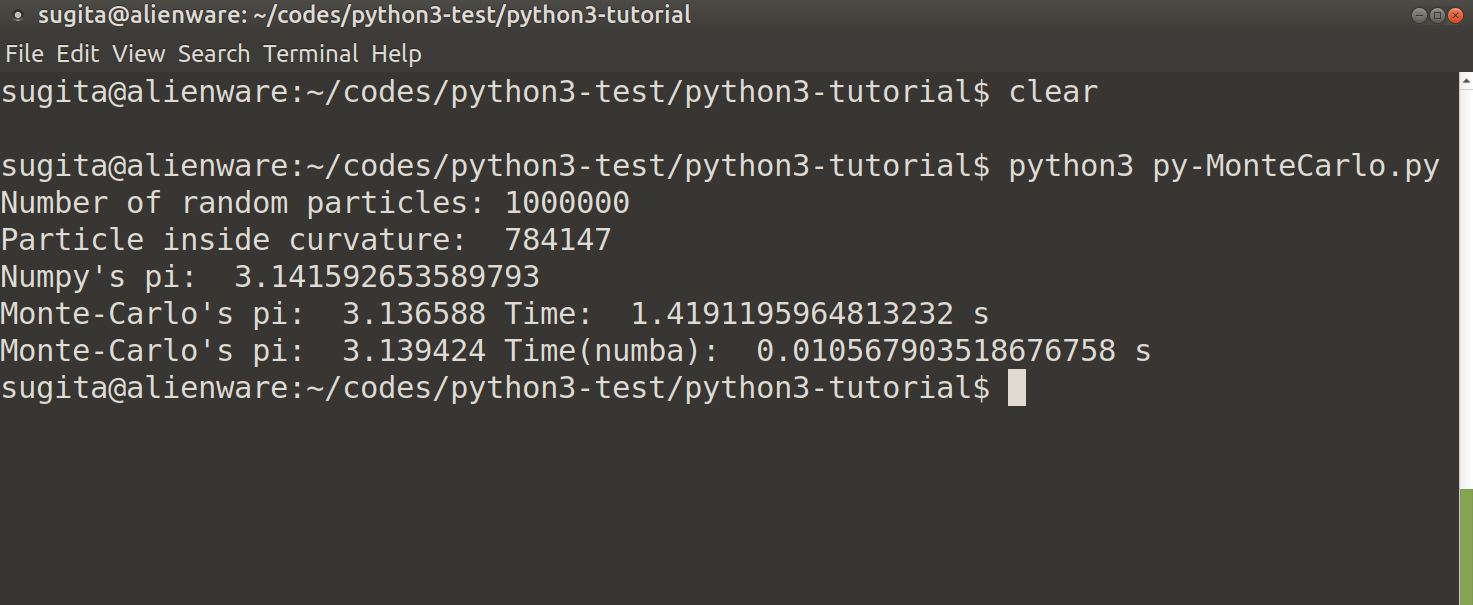
\includegraphics[width=\textwidth]{numba-vs-normal.png}
\caption{Numba vs normal script computation time.}
\end{figure}
\end{itemize}
\end{frame}

\begin{frame}
\Huge{\centerline{Thank You!}}
\Huge{\centerline{Questions?}}
\end{frame}

\end{document} 